%%% Local Variables:
%%% mode: latex
%%% TeX-master: "../index"
%%% End:

\subsection{Symmetric-key algorithms}
\unfootnote{\url{http://en.wikipedia.org/wiki/Symmetric-key_algorithm}}

\subsubsection{Overview}
\begin{itemize}
\item \textbf{Class of algorithms} for cryptography that use the same
  cryptographic keys for both encryption of plaintext and decryption
  of ciphertext.
\item The keys may be \textbf{identical} or there may be a \textbf{simple
  transformation} to go between the two keys.
\item The keys, in practice, represent a \textbf{shared secret} between two or
  more parties that can be used to maintain a private information
  link.
\item This requirement that both parties have access to the secret key
nn  is one of the \textbf{main drawbacks} of symmetric key encryption, in
  comparison to public-key encryption.
\end{itemize}

\subsubsection{Types}
Symmetric-key encryption can use either stream ciphers or block ciphers:
\begin{itemize}
\item \textbf{Stream ciphers} encrypt the digits (typically bytes) of a
  message one at a time.
\item \textbf{Block ciphers} take a number of bits and encrypt them as a
  single unit, padding the plaintext so that it is a multiple of the
  block size. Blocks of 64 bits have been commonly used (AES uses
  128-bit blocks).
\end{itemize}

\subsection{Cryptanalysis}

We make the following \textbf{assumptions}:
\begin{itemize}
\item All keys are equally likely and a key $k$ is always chosen
  uniformly at random.
\item \textbf{Kerckhoffs’ Assumption}: The attack knows all details of
  the enciphering process and deciphering process except for the
  value of the secret key.
\end{itemize}

\subsubsection{Types of Attack}

\begin{description}
\item[Ciphertext only attack]:\\
  The attacker intercepts a set of ciphertexts.
\item[Known plaintext attack]:\\
  The attacker obtains a set of s plaintexts $m_1 , m_2 , \ldots, m_s$
  and the corresponding ciphertexts $c_1 , c_2 , \ldots, c_s$. That
  is, the attacker has no control over the pairs of plaintexts and
  ciphertexts available to him.
\item[Chosen plaintext attack]:\\
  The attacker chooses a priori set of $s$ plaintexts $m_1 , m_2 ,
  \ldots, m_s$ and obtains in some way the corresponding ciphertexts
  $c_1 , c_2 , \ldots, c_s$.
\item[Adaptively chosen plaintext attack]:\\
  The attacker chooses a set of plaintexts $m_1 , m_2 , \ldots, m_s$
  interactively as he obtains the corresponding ciphertexts $c_1 , c_2
  , \ldots, c_s$. That is, the attacker chooses $m_1$, obtains $c_1$,
  then chooses $m_2$ etc.
\item[Chosen ciphertext attacks]:\\
  These are similar to the chosen plaintext attacks and adaptively
  chosen plaintext attacks, where the roles of plaintext and
  ciphertext are swapped.
\end{description}

The ultimate goal of the attacker is to find the secret key, but this
is not always necessary. For example, the attacker might be able to
find the plaintexts in a ciphertext-only attack without knowing (all
of) the secret key.

\subsection{Old systems}
\subsubsection{Shift / Caesar}
Key $K \in \mathbb{Z}_{26}$
\[ e_k(m_i) =  m_i + k \mod 26 \]
\[ d_k(c_i) = c_i - k \mod 26 \]

\subsubsection{Affine}
Key $K = (a \times b) \in (\mathbb{Z}_{26}^* \times \mathbb{Z}_{26}$)

\[ e_k(m_i) = a \cdot m_i + k \mod 26 \]
\[ d_k(c_i) = a^{-1}(c_i - b) \mod 26 \]

$a$ must have a multiplicative inverse ($a^{-1}$)

\subsubsection{Vigenere}
\[ e_k (m) = (m_0 + k_0, m_1 + k_1, \ldots, m_{j-1} + k_{j-1} ) \mod 26 \]
\[ d_k (c) = (c_0 - k_0 , c_1 - k_1 , \ldots, c_{j-1} - k_{j-1} ) \mod 26 \]

Message $m$ is split into blocks of same length as key $k$ if $length(m) > length(k)$

\subsubsection{Hill}
Key is a $j \times j$ \emph{invertible} matrix over $\mathbb{Z}_{26}$. Message $m$ is regarded as vectors of length $j$.

\begin{figure}[H]
\centering
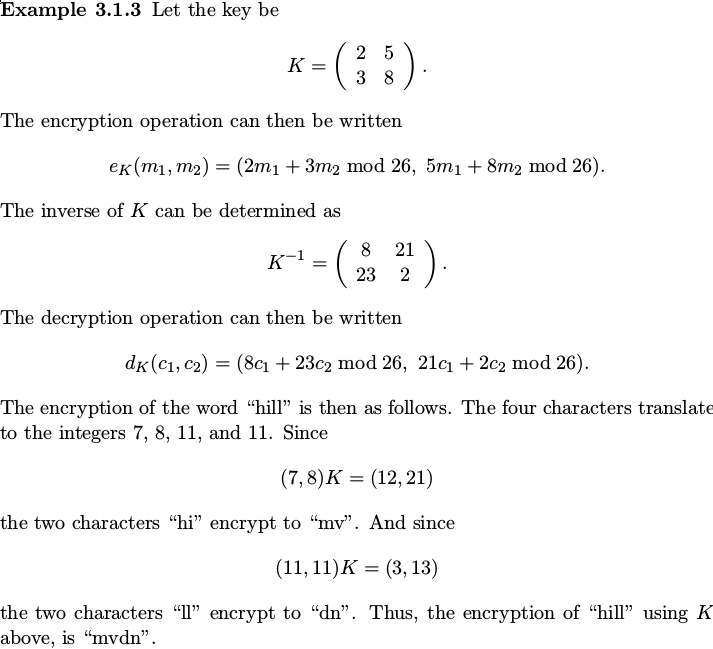
\includegraphics[scale=0.3]{images/1-hill.png}
\caption{Example of Hill cipher enc/dec}
\end{figure}
